\documentclass[10pt,a4paper]{article}

\usepackage[margin=1.45cm]{geometry}
\usepackage[T1]{fontenc}
\usepackage[utf8]{inputenc}
\usepackage{lmodern}
\usepackage{microtype}
\usepackage{graphicx}
\usepackage{booktabs}
\usepackage{tabularx}
\usepackage{array}
\usepackage{enumitem}
\usepackage{xcolor}
\usepackage{hyperref}
\usepackage{tikz}
\usetikzlibrary{arrows.meta,positioning,shapes.geometric}

\hypersetup{
  colorlinks=true,
  linkcolor=black,
  urlcolor=blue!50!black
}

\setlength{\parindent}{0pt}
\setlength{\parskip}{0.18em}
\setlength{\textfloatsep}{6pt plus 2pt minus 2pt}
\setlength{\floatsep}{6pt plus 2pt minus 2pt}
\setlength{\intextsep}{6pt plus 2pt minus 2pt}
\setlength{\abovecaptionskip}{3pt}
\setlength{\belowcaptionskip}{0pt}
\setlist[itemize]{leftmargin=*, itemsep=0.1em, topsep=0.1em}
\setlist[enumerate]{leftmargin=*, itemsep=0.1em, topsep=0.1em}

\title{\vspace{-1.2em}\textbf{FPGA Wand: A Multi-Node PYNQ-to-Cloud Interactive Drawing System}\vspace{-0.6em}}
\author{Group 10}
\date{}

\begin{document}
\maketitle
\vspace{-1.4em}
\begin{center}
\small Repository and run instructions: \url{https://github.com/dydx404/fpga_wand}
\end{center}
\vspace{-0.7em}

\section{Purpose and Final System}

The aim of this project was to build a multi-node information-processing system
in which FPGA SoC devices perform local processing, communicate with a cloud
server, and receive information back from the server in a way that changes
node-side behaviour. The delivered system, \emph{FPGA Wand}, satisfies this
brief through two PYNQ-Z1 nodes, each equipped with a camera observing a bright
wand tip, and an EC2-hosted backend called \emph{Wand Brain}. Each node reduces
the incoming camera frames to compact point events locally and transmits them to
the cloud over UDP. The backend reconstructs strokes, renders live and
finalized drawings, scores completed attempts against templates, stores results
in a database, and serves a browser dashboard over HTTP. The same HTTP path is
also used to influence node-side behaviour through revisioned runtime control.

The final system therefore covers all minimum functional requirements:
meaningful local processing on the FPGA SoC, a cloud server that processes
events, communication from node to server, communication from server back to
node, and successful concurrent use of two nodes. It also extends the brief
through a template-based game layer that includes recent-attempt history,
leaderboards, named template champions, and a live operator console. The
project is consequently better understood as an end-to-end interactive system
than as a simple transport demonstration.

\section{Overall Architecture}

\begin{figure}[t]
\centering
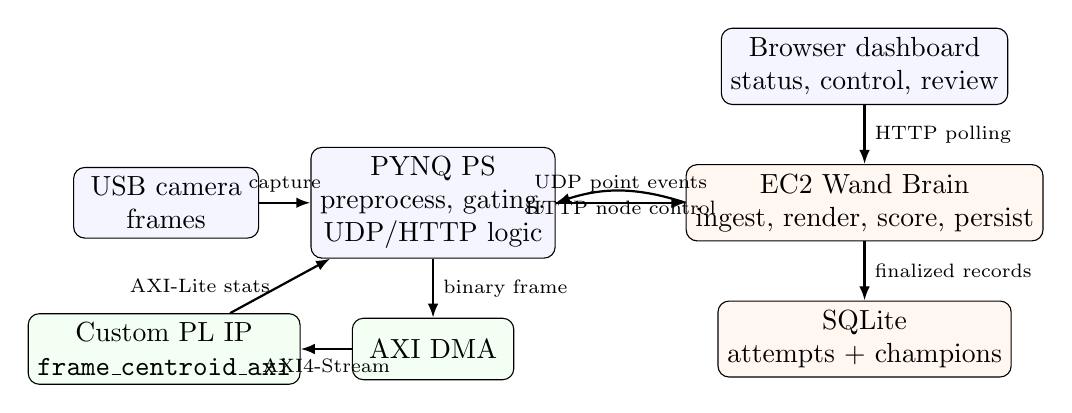
\begin{tikzpicture}[
  node distance=0.75cm and 0.65cm,
  box/.style={draw, rounded corners, align=center, minimum width=2.35cm, minimum height=0.85cm, fill=blue!4},
  smallbox/.style={draw, rounded corners, align=center, minimum width=2.05cm, minimum height=0.78cm, fill=green!5},
  cloudbox/.style={draw, rounded corners, align=center, minimum width=2.65cm, minimum height=0.9cm, fill=orange!6},
  line/.style={-{Latex[length=1.8mm]}, thick}
]
\node[box] (camera) {USB camera\\frames};
\node[box, right=of camera] (ps) {PYNQ PS\\preprocess, gating,\\UDP/HTTP logic};
\node[smallbox, below=of ps] (dma) {AXI DMA};
\node[smallbox, left=of dma] (pl) {Custom PL IP\\\texttt{frame\_centroid\_axi}};
\node[cloudbox, right=of ps, xshift=1cm] (brain) {EC2 Wand Brain\\ingest, render, score, persist};
\node[cloudbox, below=of brain] (db) {SQLite\\attempts + champions};
\node[box, above=of brain] (web) {Browser dashboard\\status, control, review};

\draw[line] (camera) -- node[above, font=\scriptsize] {capture} (ps);
\draw[line] (ps) -- node[right, font=\scriptsize] {binary frame} (dma);
\draw[line] (dma) -- node[below, font=\scriptsize] {AXI4-Stream} (pl);
\draw[line] (pl) -- node[left, font=\scriptsize] {AXI-Lite stats} (ps);
\draw[line] (ps) -- node[above, font=\scriptsize] {UDP point events} (brain);
\draw[line] (brain) -- node[right, font=\scriptsize] {finalized records} (db);
\draw[line] (web) -- node[right, font=\scriptsize] {HTTP polling} (brain);
\draw[line] (brain.west) to[bend right=18] node[below, font=\scriptsize] {HTTP node control} (ps.east);
\end{tikzpicture}
\caption{Adopted end-to-end architecture. The final system separates a UDP
point-stream data plane from an HTTP control, persistence, and presentation
plane.}
\label{fig:system-architecture}
\end{figure}

Figure~\ref{fig:system-architecture} shows the final architecture. The local
node combines the Zynq Processing System (PS) and Programmable Logic (PL), but
the design is intentionally not ``all hardware''. The PL performs a narrow,
deterministic reduction task, while the PS retains the policy-heavy parts of
the runtime. The backend mirrors this design style: a compact real-time core
handles ingest and live reconstruction, while a wrapper layer provides
persistence, node control, and the web interface.

\subsection*{Node-side hardware and local processing}

Each node is built around a PYNQ-Z1 board, an Arducam B0332 camera using the
OV9281 monochrome global-shutter sensor, a USB hub, and a WiFi adapter. This
hardware choice was important to the success of the final system. The camera is
well suited to fast target tracking because it supports high-frame-rate MJPG
capture, uses a global shutter to reduce motion distortion, and has no IR cut
filter, which keeps it sensitive to near-infrared light. The optical chain was
also treated as part of the design problem: a camera mount and IR-filter holder
were documented so that visible-light leakage into the optical path could be
reduced. The wand itself was simplified to a bright handheld LED target with a
custom enclosure and battery-powered illumination. This hardware simplification
reduced the burden on later computational stages.

\begin{figure}[t]
\centering
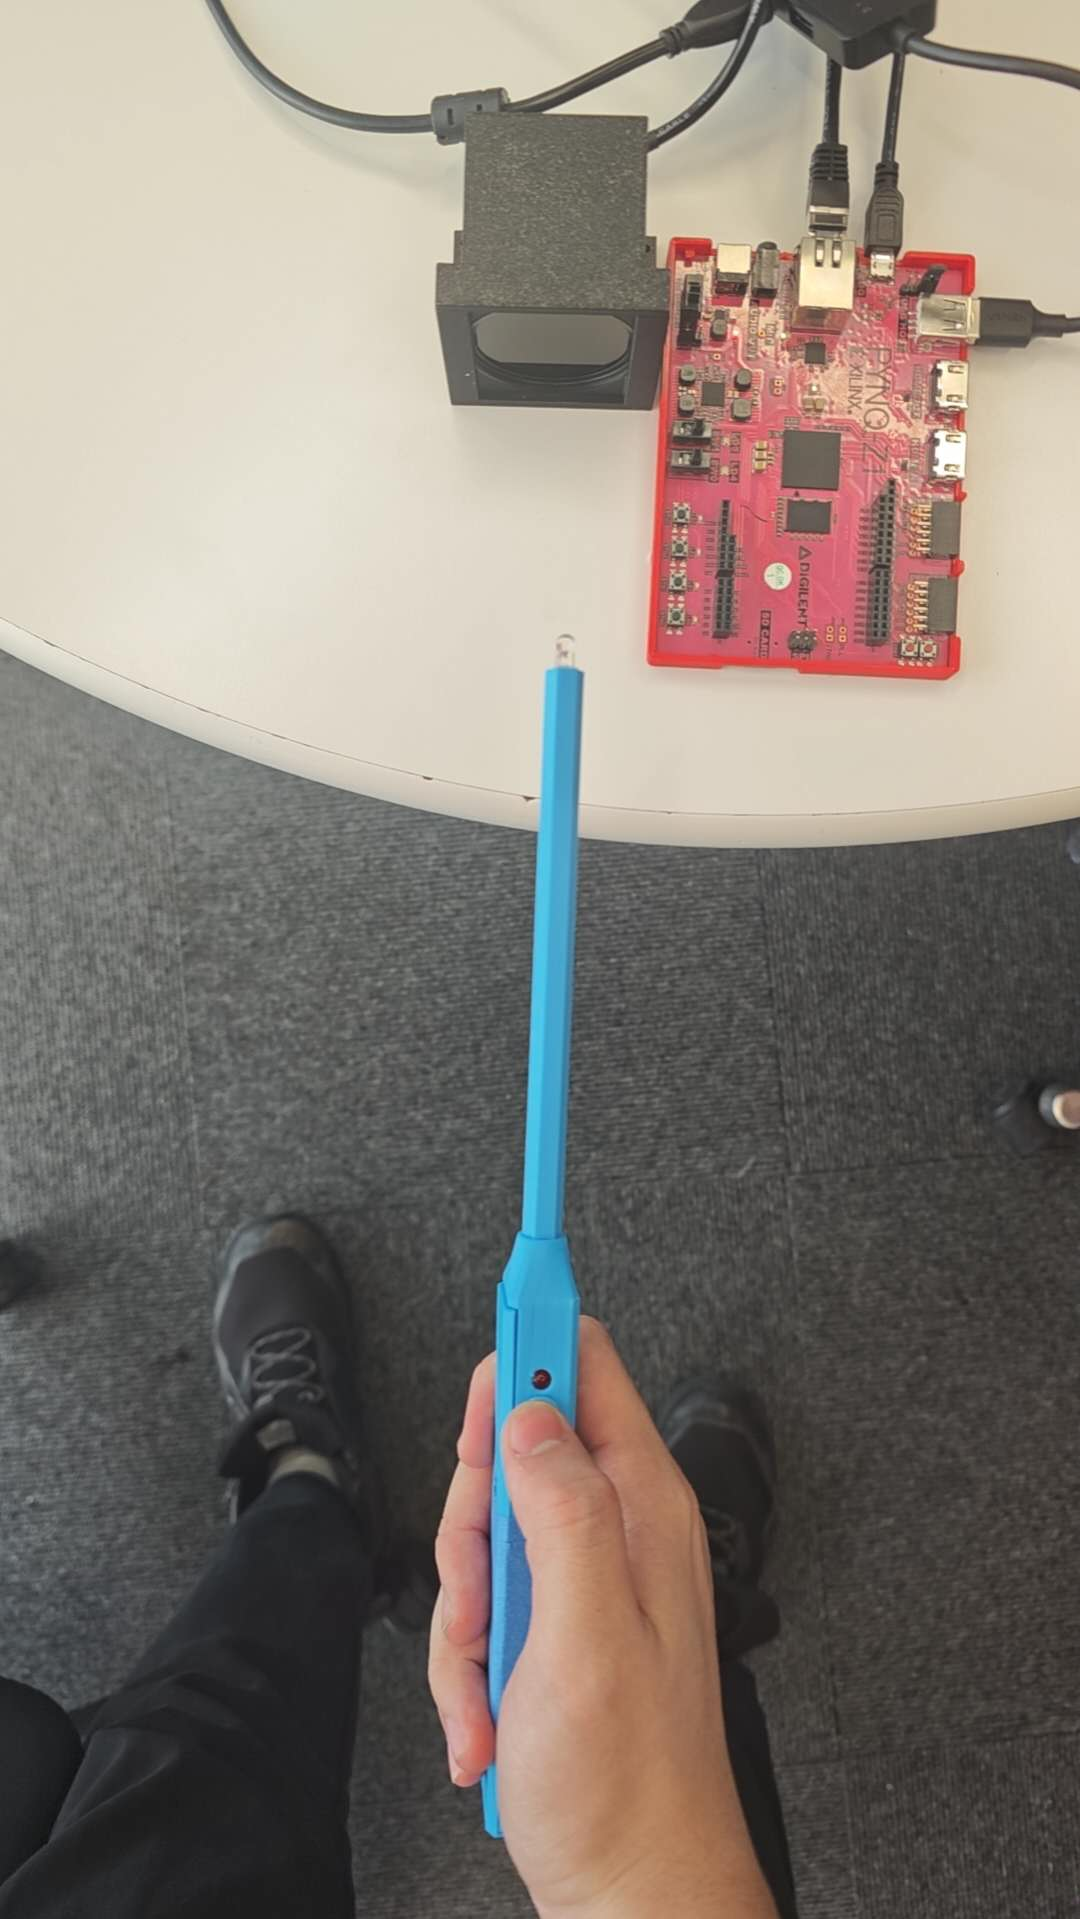
\includegraphics[width=0.30\linewidth]{../../docs/pictures and videos/full_hardware.jpg}
\caption{Physical prototype used in the final system demonstration. The setup
combines the PYNQ node, optical tracking hardware, and the illuminated wand
used by the local processing pipeline.}
\label{fig:hardware-photo}
\end{figure}

At runtime, the PS opens and warms the camera, loads the bitstream, discovers
the DMA and centroid IP blocks from the overlay, opens an AXI-Lite MMIO window,
allocates a contiguous frame buffer, creates the UDP/HTTP bridge, and performs
an initial backend health and control check. For every frame, the PS captures a
BGR image, converts it to grayscale, resizes it to $640\times480$, applies a
small blur, and thresholds it into a binary mask. That binary frame is flattened
into a DMA buffer and streamed through \texttt{axi\_dma\_0} into the custom PL
block \texttt{frame\_centroid\_axi}. The PL consumes 32-bit AXI stream words,
equivalent to four 8-bit pixels per beat, and accumulates only the compact
statistics required for centroid estimation: $\sum x$, $\sum y$, foreground
pixel count, frame ID, and a valid flag. The result returns to the PS over a
small AXI-Lite register interface rather than as another image stream.

This PS/PL boundary is central to the project. The PL performs the regular,
repeated per-pixel arithmetic, while the PS performs centroid division, point
acceptance, runtime filtering, line continuity, network packet generation, and
server-control handling. This split proved robust because the software-side
policy changed several times during integration, whereas the compact
centroid-style hardware stage remained stable.

\subsection*{Node-to-cloud communication and control}

The node-to-cloud protocol is the fixed-size UDP format
\texttt{wb-point-v1}. Each packet is 24 bytes and carries one point sample
together with device number, wand ID, packet number, stroke ID, timestamp, and
stroke-state flags such as \texttt{STROKE\_START}, \texttt{PEN\_DOWN}, and
\texttt{STROKE\_END}. Coordinates are sent in a compact Q15 representation
rather than as pixels, so the cloud never receives camera images directly. This
keeps the network path lightweight and makes the backend independent of camera
resolution.

The reverse path, from server to node, uses revisioned HTTP control objects.
Each node polls its control endpoint and can receive changes to values such as
\texttt{enabled}, \texttt{armed}, \texttt{tx\_enabled}, threshold,
\texttt{min\_count}, gap timeout, and smoothing mode. The node then posts an
acknowledgement that records the applied revision and whether a change is still
pending. This control structure allowed the backend to influence local
processing directly, which was a required part of the brief, while still
keeping the high-frequency point path on UDP.

\section{Wand Brain Backend}

The backend is implemented as a FastAPI application on EC2 and is organised in
two layers. The inner layer is the live \emph{Brain} runtime. It receives UDP
traffic on port 41000, parses packets, reconstructs active attempts in memory,
renders live images, and finalizes attempts. The outer wrapper layer adds
SQLite-based persistence, template selection, node-control APIs, recent-attempt
views, and the single-page dashboard served on port 8000. This separation keeps
the real-time path small while still exposing a richer application surface.

Packet parsing is intentionally narrow in responsibility. The parser checks the
24-byte length, validates the magic number and version, confirms that the
encoded coordinates are within the expected range, and decodes the flags into a
typed point event. The more important logic sits one level above this: the
\texttt{BrainState} runtime decides whether a packet extends the current attempt
or starts a new one, appends the point to the in-memory buffer, updates per-wand
status, and finalizes the attempt on either an explicit end packet or an idle
timeout. This distinction is important architecturally. The parser answers
``what does this packet contain?'', whereas the runtime answers ``what does this
event mean for the current drawing state?''.

Live plotting is handled by rasterizing the buffered points into a fixed
$256\times256$ viewport during an active stroke. This fixed mapping is a useful
detail because it avoids zooming and reframing the drawing while the user is
still drawing. When an attempt finalizes, the backend saves a finalized PNG,
records timing and point-count information, and passes the image into the
scoring stage. The scoring method is deliberately transparent: both the drawing
and the selected template are converted to binary $256\times256$ images, then
three overlap-style measures are calculated, namely Dice coefficient,
intersection-over-union, and an area-ratio term that penalizes large size
mismatch. The final score is a weighted combination,
\[
\mathrm{score} = 100 \times (0.55\,\mathrm{Dice} + 0.35\,\mathrm{IoU} + 0.10\,\mathrm{AreaRatio}).
\]
This is simpler than a full recognition pipeline, but it is deterministic,
cheap to compute, and easy to explain during live use.

Persistence is downstream of the live runtime rather than part of the hot ingest
path. Active attempts remain in memory until they finalize. At that point, the
wrapper writes a row into the \texttt{Attempt} table containing wand identity,
attempt ID, start and end time, finalized time, point count, render path, and
the best template score. Template leaders are stored separately in the
\texttt{TemplateChampion} table, which records only the current champion per
template rather than a full ranking history. This database design is small but
appropriate: it preserves meaningful application results without paying a write
cost for every incoming point event.

The final backend also distinguishes carefully between source identity from the
node and backend-owned identity used for persistence. The UDP stream contains a
\texttt{stroke\_id} generated by the node, but the backend assigns its own
internal attempt identifier when reconstructing a live drawing. This proved
important in practice, because source stroke IDs could be reused after a board
restart, while database and history views require a stable unique identifier
under backend control. The same lifecycle logic is used for stroke closure: an
attempt may end on an explicit \texttt{STROKE\_END} packet or after a short idle
timeout, which allows the system to tolerate brief input gaps without breaking
every stroke into many fragments.

The dashboard itself is intentionally simple. It is a single HTML page with
embedded JavaScript and no heavy frontend framework. The page polls the backend
at different intervals depending on the type of data. The live image and wand
status are refreshed quickly, while database-backed content such as recent
attempts and leaderboards is refreshed more slowly. This simplified deployment
considerably and made debugging straightforward, because the operator and the
browser relied on exactly the same HTTP endpoints.

\begin{figure}[t]
\centering
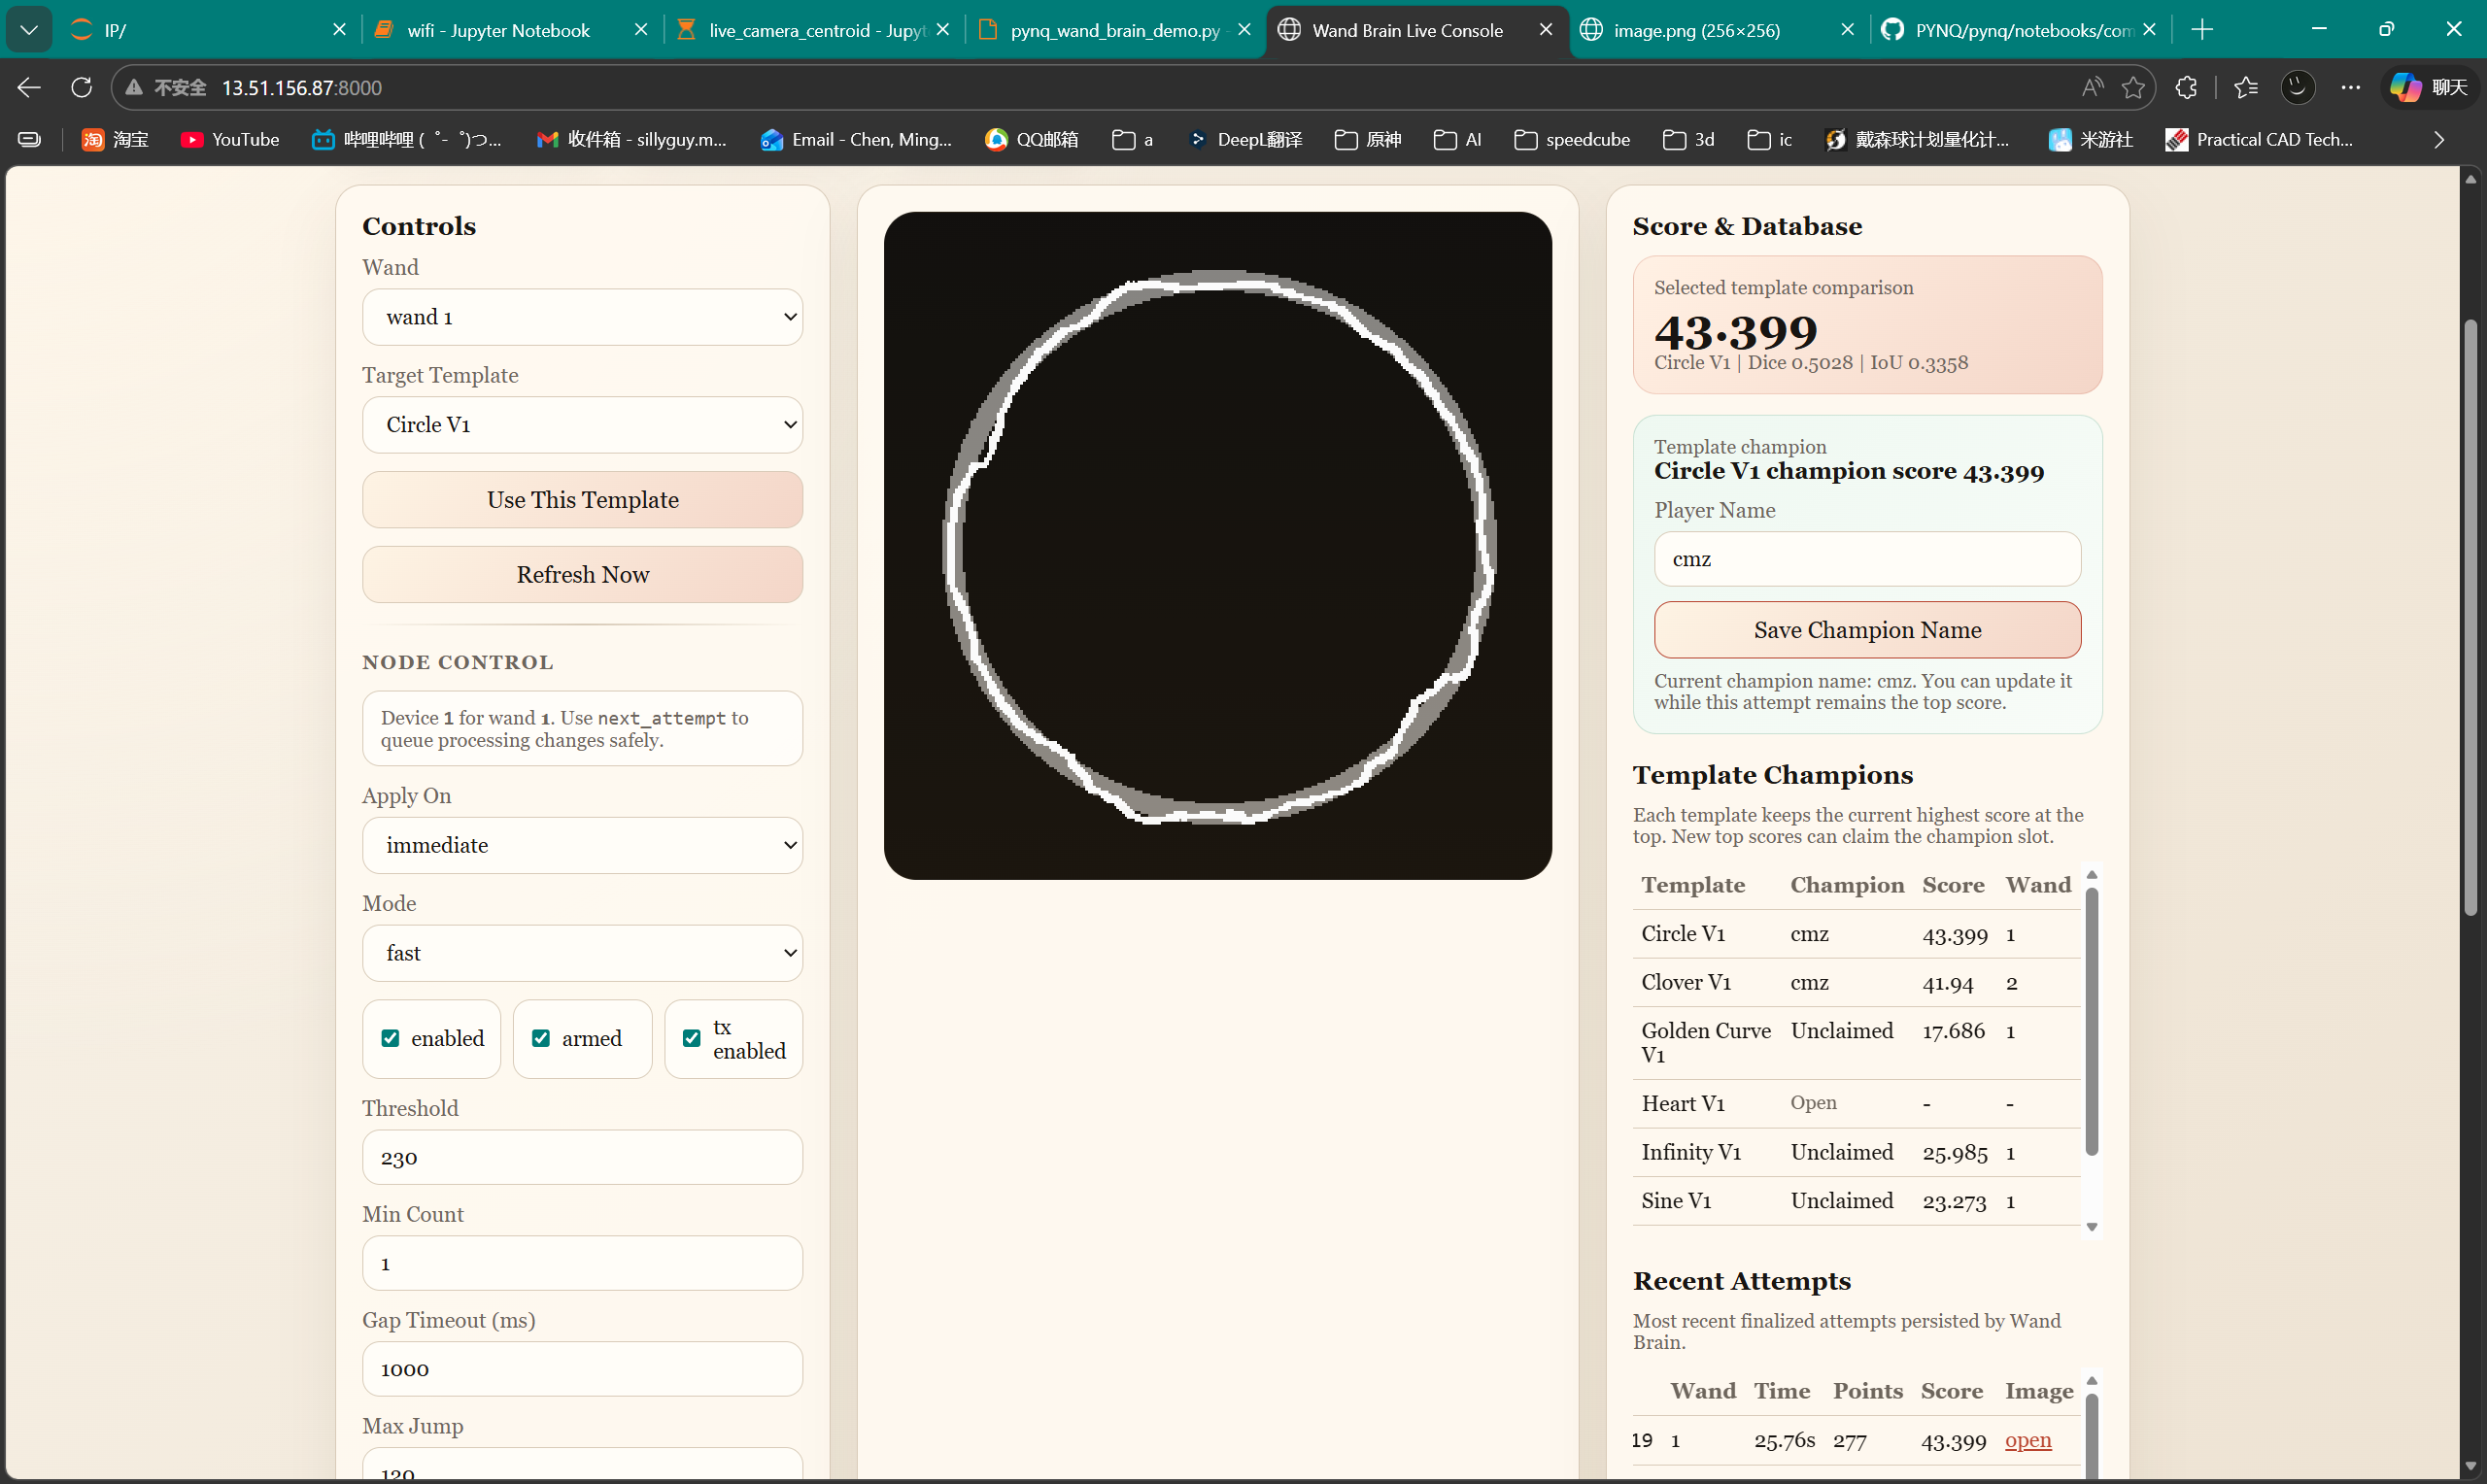
\includegraphics[width=0.39\linewidth]{../../docs/pictures and videos/higher_website.png}
\caption{The deployed Wand Brain dashboard. The interface combines live
visualization, node control, score inspection, recent-attempt history, and
leaderboard review inside a single operator page.}
\label{fig:dashboard}
\end{figure}

Another important backend characteristic is that template selection, scoring,
and persistence are linked directly to the attempt lifecycle. When a template is
selected for a wand, that association is remembered for the current or next
attempt. When finalization occurs, the backend renders the final stroke image,
computes the overlap-based score against the selected template, and writes the
scored result into the database. The leaderboard layer is then updated only if
that attempt exceeds the existing champion score for the template. This keeps
the gameplay logic consistent with the runtime model: scoring happens when an
attempt becomes complete and durable, not during partial drawing.

The backend also improves observability by exposing separate views for health,
database status, live wand state, recent attempts, node-control state, and
leaderboards. This mattered in practice because it allowed faults to be
localized quickly. For example, a healthy database with an inactive live wand
suggests a node-side issue, while healthy live status but missing recent rows
suggests a persistence or ordering problem.

This observability model is also reflected in the webpage update strategy. Fast
polling is used only where immediacy matters, such as live image refresh and
wand status, while lower-frequency polling is used for database-backed views
that change only after attempt finalization. That split reduced unnecessary
request traffic and made the operator console readable: the centre panel stays
responsive during drawing, while score, leaderboard, and recent-attempt panels
update at a human-facing pace.

From a systems perspective, this webpage is more than a presentation layer. It
was used as an operational debugging surface during integration. Control-state
summaries, acknowledgement views, health badges, timer displays, and historical
tables all exposed internal backend state in a form that was easy to compare
with live physical behaviour. This reduced the gap between engineering
instrumentation and final demonstration interface, which was especially useful
late in the project when rapid iteration on thresholds, packet handling, and
attempt lifecycle behaviour was still taking place.

\section{Performance Metrics and Design Decisions}

\begin{table}[t]
\centering
\footnotesize
\begin{tabularx}{\linewidth}{>{\raggedright\arraybackslash}p{2.8cm} >{\raggedright\arraybackslash}p{3.7cm} X}
\toprule
\textbf{Metric} & \textbf{Reason for use} & \textbf{Evidence in the final system} \\
\midrule
Stroke correctness & The physical motion must remain recognisable after local reduction, transmission, and reconstruction. & Verified through live rendering, finalized PNGs, and template scoring using the real camera and wand. \\
Interaction responsiveness & The system must remain usable as an interactive drawing platform rather than only as an offline processor. & Small UDP packets, local point gating, fixed-size live rasterization, and fast dashboard polling supported responsive updates. \\
Two-node isolation & The brief requires more than one active node. & Distinct \texttt{device\_number} and \texttt{wand\_id} values were preserved across the protocol, backend state, and dashboard. \\
Server control correctness & The cloud must influence local behaviour, not only observe it. & HTTP control revisions changed node mode, threshold, transmission state, and recalibration behaviour. \\
Deployable FPGA implementation & Hardware acceleration should help without becoming an integration bottleneck. & The adopted PL path remained compact, streamed four pixels per beat, and closed timing successfully. \\
\bottomrule
\end{tabularx}
\caption{Performance metrics used to evaluate the project.}
\label{tab:metrics}
\end{table}

These metrics reflect the fact that the project is a distributed interactive
system rather than a pure throughput benchmark. A very high frame rate would
not be sufficient if strokes were fragmented, if packet identity was handled
incorrectly, or if the server could not safely influence node-side behaviour.
For this reason, the evaluation emphasises the correctness of the integrated
capture-to-score path and the reliability of the two-way control architecture.

Several design decisions follow directly from this evaluation logic. The first
is the selective use of hardware. Instead of forcing the entire vision pipeline
into the PL, the final system accelerates the regular per-pixel reduction stage
and leaves policy-heavy logic in software. This reduced integration cost while
still using the FPGA fabric meaningfully. The second is the separation of
protocol responsibilities: UDP carries only the time-sensitive point stream,
whereas HTTP carries control, acknowledgements, templates, leaderboards, and
dashboard data. The third is the split between live in-memory state and
database-backed historical state. This keeps active strokes cheap to update
while preserving finalized results for review and gameplay features.

The physical sensing chain is also part of the design evaluation. The choice of
a bright optical target, a monochrome global-shutter camera, and IR-aware
mounting improved the computational problem presented to the node. This is an
important systems point: robustness was not achieved only through software or
hardware acceleration, but through a design that made the input easier to
segment in the first place. The backend follows the same principle by storing
only finalized attempts rather than every incoming point, thereby reducing
state volume before it becomes a maintenance burden.

\section{Testing Approach}

\begin{figure}[t]
\centering
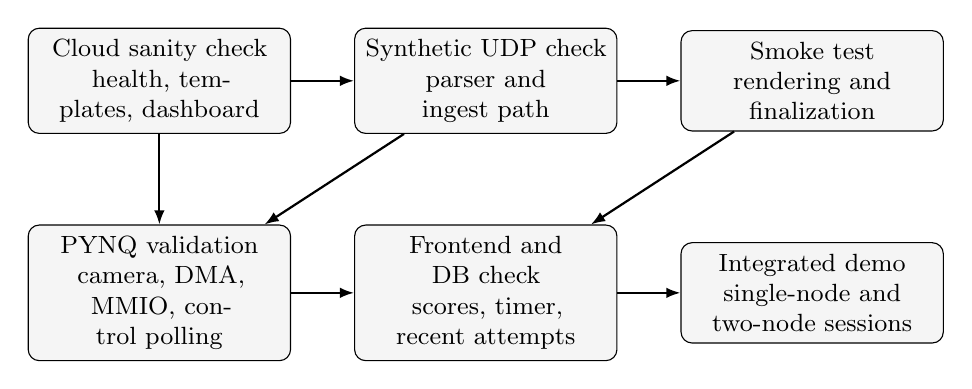
\begin{tikzpicture}[
  node distance=1.05cm and 0.8cm,
  stepbox/.style={
    draw,
    rounded corners,
    align=center,
    text width=3.05cm,
    minimum height=0.9cm,
    inner sep=4pt,
    font=\small,
    fill=gray!8
  },
  flow/.style={-{Latex[length=1.8mm]}, thick}
]
\node[stepbox] (cloud) {Cloud sanity check\\health, templates, dashboard};
\node[stepbox, right=of cloud] (udp) {Synthetic UDP check\\parser and ingest path};
\node[stepbox, right=of udp] (smoke) {Smoke test\\rendering and finalization};
\node[stepbox, below=1.15cm of cloud] (board) {PYNQ validation\\camera, DMA, MMIO, control polling};
\node[stepbox, right=of board] (ui) {Frontend and DB check\\scores, timer, recent attempts};
\node[stepbox, right=of ui] (multi) {Integrated demo\\single-node and two-node sessions};

\draw[flow] (cloud) -- (udp);
\draw[flow] (udp) -- (smoke);
\draw[flow] (cloud) -- (board);
\draw[flow] (udp) -- (board);
\draw[flow] (smoke) -- (ui);
\draw[flow] (board) -- (ui);
\draw[flow] (ui) -- (multi);
\end{tikzpicture}
\caption{Testing flow used to move from isolated subsystem checks to full
end-to-end validation.}
\label{fig:test-flow}
\end{figure}

Testing followed the staged approach shown in Figure~\ref{fig:test-flow}. This
was necessary because the project had several failure boundaries: camera and
PL, node-side runtime logic, UDP transport, backend reconstruction, persistence,
and browser presentation.

Cloud-only testing covered health endpoints, template enumeration, synthetic UDP
injection, live image generation, and finalized-attempt rendering. Board-level
testing covered camera bring-up, repeated DMA transfers, changing MMIO results,
backend reachability, and node-control acknowledgements. Integrated testing was
then performed using the deployed EC2 backend, the actual PYNQ nodes, and the
live dashboard. The final validated behaviours included live plotting,
finalized scoring, recent-attempt updates, leaderboard updates, server-to-node
control through the HTML panel, and successful one-node and two-node sessions.

This staged process also exposed integration issues that would not have been
visible from isolated unit checks. Examples included camera startup fragility,
the need to separate backend-owned attempt IDs from incoming source stroke IDs,
the need to sort recent attempts by finalization time rather than creation
time, and the need to retune thresholding under changing lighting. The fact
that these issues were resolved without a full redesign indicates that the
chosen architectural boundaries were sound.

The testing strategy also maps directly onto the functional requirements of the
brief. Local processing was verified through camera capture, preprocessing,
DMA, and MMIO readback on the node; cloud processing was verified through live
ingest, rendering, scoring, and persistence; node-to-server communication was
verified through UDP packet injection and real-board traffic; server-to-node
communication was verified through the HTTP control panel and acknowledgement
routes; and the multi-node requirement was verified through integrated two-node
operation against the same deployed backend.

\section{FPGA Implementation and Device Resources}

\begin{figure}[t]
\centering
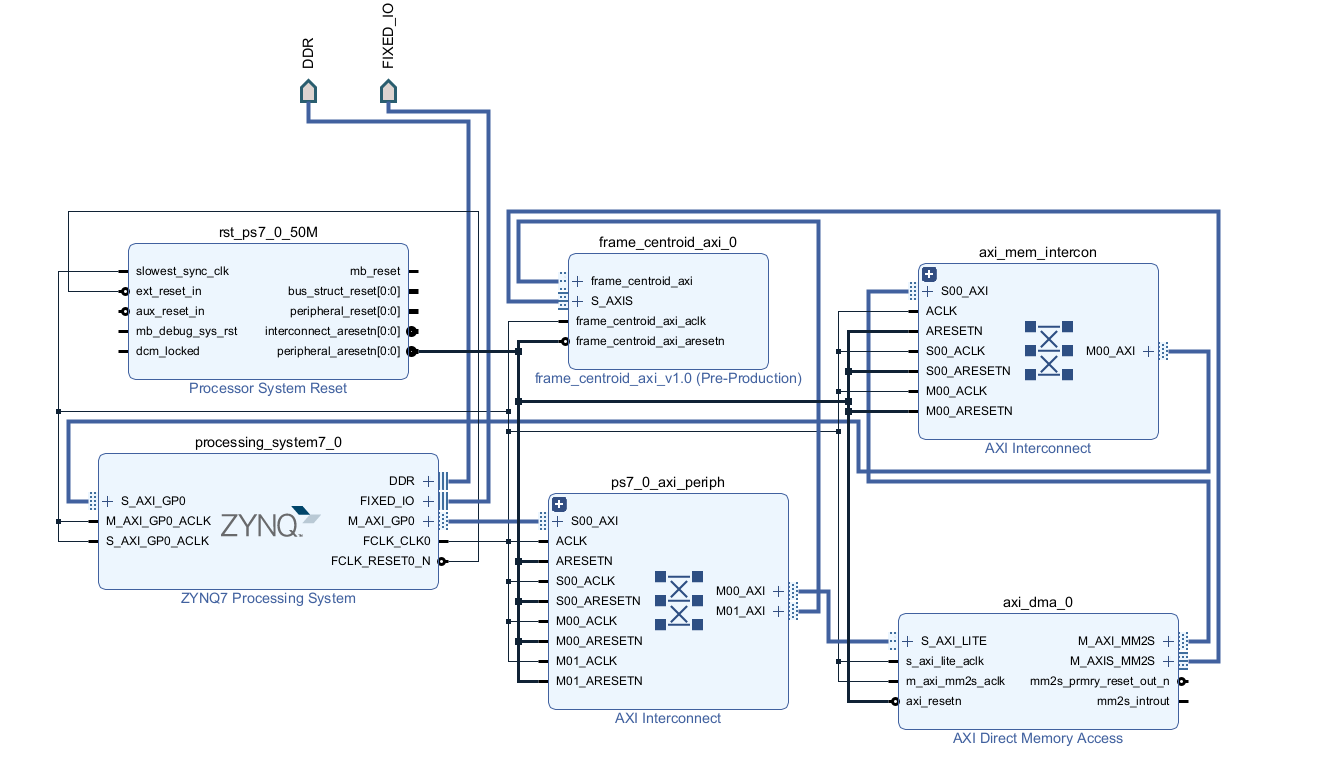
\includegraphics[width=0.34\linewidth]{../../FPGA/designs/centroid_pipeline/used_version/images/top.png}
\caption{Top-level adopted FPGA design. The PS controls memory, DMA, and AXI-Lite
register access, while the custom IP performs the centroid-style reduction over
the streamed binary frame.}
\label{fig:fpga-top}
\end{figure}

The adopted FPGA implementation is intentionally narrow. The custom IP accepts a
binary image stream and performs only the foreground reduction task. It does not
implement connected-component analysis, frame-scale storage, hardware division,
or higher-level stroke logic. The data path is one-way: DDR memory to AXI DMA,
AXI DMA to AXI4-Stream, AXI stream into the custom IP, and compact statistics
back to the PS over AXI-Lite. In that sense, the device resources are used
selectively rather than maximally.

This resource strategy is the main hardware trade-off in the project. A more
ambitious PL path was explored earlier, but the final centroid pipeline was
chosen because it accelerates the most regular part of the workload while
keeping the rest of the system easy to modify. As a result, thresholding
policy, stroke-gap handling, smoothing, and network behaviour remained software
operations on the PS and could still be tuned late in development.

An earlier FPGA path, developed by Wells, explored a broader stream-processing
architecture based around convolution filtering, line buffers, and a more
ambitious image-processing chain before centroid extraction. That work was
useful in surfacing practical issues around AXI-stream integration, DMA
behaviour, and hardware debugging, but it was not adopted as the final delivery
path. In the final system, the narrower centroid-based design was preferred
because it was easier to integrate reliably with the PS runtime and the
cloud-facing communication stack.

In technical terms, that earlier design aimed at a richer hardware pipeline:
input video stream, pixel downsampling, convolution-based filtering, logical-map
conversion, and later centroid extraction. The custom HDL in that branch
implements the convolution-filter stage using line buffers and a streaming
kernel-style architecture, and simulation evidence was retained for that
subsystem. The main unresolved issue reported for that path was in the DMA
receive side, where the returned frame data did not match the transmitted size.
From the perspective of the final report, this alternative path is important
because it shows that the final adopted design was a deliberate architectural
choice rather than the only idea attempted.

The repository retains timing-closure evidence for the implemented design. The
archived timing summary reports setup slack of 11.636\,ns, hold slack of
0.045\,ns, pulse-width slack of 8.750\,ns, and zero failing endpoints. A full
post-implementation LUT/FF/BRAM table was not retained in the repository, so
this report does not claim unsupported utilization numbers. The stronger
defensible statement is architectural: the final PL scope was deliberately
limited to stream arithmetic and accumulation, and that compact scope produced a
design that closed timing on the target board and integrated reliably with the
rest of the system.

This final FPGA choice should therefore be understood as an optimisation in the
sense intended by the module: it applies hardware acceleration where the
workload is regular and repeated, but leaves rapidly changing policy decisions
in software where they can be tuned safely. In that sense, the most important
resource result is not simply that a custom IP was built, but that the final
hardware/software partition remained stable enough to support the cloud-facing
features, testing process, and final two-node demonstration.

\section{Conclusion}

The final project delivered a complete multi-node FPGA-to-cloud information
processing system. Each PYNQ node performed local preprocessing and FPGA-backed
centroid reduction, sent compact point events to the cloud over UDP, and
received runtime control back from the server over HTTP. The Wand Brain backend
reconstructed strokes, rendered live and finalized drawings, scored attempts
against templates, persisted results, and served a live dashboard. The final
system demonstrated successful single-node and two-node operation and therefore
met the coursework objectives in a balanced and technically defensible way.

\end{document}
